%% LaTeX-Beamer template for KIT design
%% by Erik Burger, Christian Hammer
%% title picture by Klaus Krogmann
%%
%% version 2.0
%%
%% mostly compatible to KIT corporate design v2.0
%% http://intranet.kit.edu/gestaltungsrichtlinien.php
%%
%% Problems, bugs and comments to
%% burger@kit.edu

\documentclass[18pt]{beamer}
\usetheme{kit}

%% TITLE PICTURE

% if a custom picture is to be used on the title page, copy it into the 'logos'
% directory, in the line below, replace 'mypicture' with the 
% filename (without extension) and uncomment the following line
% (picture proportions: 63 : 20, *.eps format if you use latex+dvips+ps2pdf,
% *.jpg/*.png/*.pdf if you use pdflatex)

%\titleimage{mypicture}

%% TITLE LOGO

% for a custom logo on the front page, copy your file into the 'logos'
% directory, insert the filename in the line below and uncomment it

%\titlelogo{mylogo}

% (*.eps format if you use latex+dvips+ps2pdf,
% *.jpg/*.png/*.pdf if you use pdflatex)

%% BIBTEX ICON/KEY

% if you want to see BibTeX keys in the references view instead of the symbol,
% uncomment the following line
% \usebibitemtemplate{\insertbiblabel}

% the presentation starts here

% change the following line to "ngerman" for German style date and logos
% change the following line to "english" for English style date and logos
\selectlanguage{ngerman}

\beamertemplatenavigationsymbolsempty

\usepackage{listings}
\definecolor{darkgray}{rgb}{0.95,0.95,0.95}
\definecolor{darkgreen}{rgb}{0.05,0.7,0.05}
\lstset{ language=Java,
	backgroundcolor=\color{darkgray}, 
	numbers=none, 
	keywordstyle=\color{black}\bfseries,
	tabsize=2,
	showspaces=false,               % show spaces adding particular underscores
	showstringspaces=false,         % underline spaces within strings
	showtabs=false, 
}



\title[Tutorium06]{Tutorium 06: Parallelismus und Testen}
\subtitle{Softwaretechnik im SS 2011, Tutorium 4}
\author{Jürgen Walter}
\date{\today}

\institute{Chair for Software Design and Quality}

\begin{document}

%title page
\begin{frame}
\titlepage
\end{frame}

%table of contents
\frame{
\frametitle{Was machen wir heute?}
	\tableofcontents
}

\section{Rückblick}

\frame{
\frametitle{Rückblick ÜB6}

	\begin{block}{Aufgabe 1 - Kontrollflussorientiertes Testen}
	\begin{itemize}
	\item kommt oft in der Klausur vor \pause
	\item relativ leicht verdiente Punkte!
	\end{itemize}
	\end{block}
}

\frame{
\frametitle{Rückblick ÜB6}

	\begin{block}{Aufgabe 2 -Gebietszerlegung und Synchronisation}
	\begin{itemize} \pause
	\item b) falls eine ähnliche Aufgabe in der Klausur vorkommt - versucht schnell eine Lösung zu finden \pause \\
		wenn ihr nicht schnell eine findet, macht besser andere Aufgaben zuerst \pause
	\item wichtig: wait() kann auch ``grundlos'' enden, daher sollte wait() immer in einer Schleife stehen
	\end{itemize}
	\end{block}
}


\frame{
\frametitle{Rückblick ÜB6}
	\begin{block}{Aufgabe 3 - Parallelisierung}
	\begin{itemize}
	\item Auch Parallelisierung kann in der Klausur vorkommen \pause
	\item merkt euch insbesondere die parallelen Entwurfsmuster und die wichtigsten Java Konstrukte
	\end{itemize}
	\end{block}
}

\section{Zum Aufwärmen}

\frame {
\frametitle{Wahr oder falsch?}
\begin{itemize}
	\color<2->[rgb]{0,1,0}
	\item Software unterliegt keinem Verschleiß.
	\color[rgb]{0,0,0}
	\pause
	\color<3->[rgb]{0,1,0}
	\item „Synchronisiere und Stabilisiere“ erzielt die Effektivität durch kurze Entwicklungsphasen.
	\color[rgb]{0,0,0}
	
	\pause
	\color<4->[rgb]{1,0,0}
	\item Kontrollflussorientierte Tests gehören zu den statischen Testverfahren.
	\color[rgb]{0,0,0}
	\pause
	\color<5->[rgb]{0,1,0}
	\item Bei der testgetriebenen Entwicklung dienen die Tests unter anderem zur Schnittstellendefinition
	\color[rgb]{0,0,0}
	\pause
	\color<6->[rgb]{1,0,0}
	\item Im Prozessmodell „Prototyp“ wird der Prototyp iterativ entwickelt und nach der Testphase produktiv eingesetzt und gewartet
	\color[rgb]{0,0,0}
	\pause
	\color<7->[rgb]{1,0,0}
	\item Die Signatur einer Methode besteht aus dem Methodennamen und dem Rückgabetyp
	\color[rgb]{0,0,0}


\end{itemize}
}

\section{ Parallelisierung}
\frame {
\frametitle {Matrix-Matrix-Multiplikation} 
	\begin{block} {Varianten}
	Es gibt viele Möglichkeiten, um $C = A x B$ zu berechnen
	\begin{itemize}
		\item klassisch bzw. ijk-Algorithmus
		\item ikj- oder kij-Reihenfolge
		\item Systolisch
		\item Cannon-Algorithmus
	\end{itemize}
	\end{block}
}

\frame {
\frametitle {Matrix-Matrix-Multiplikation} 
	\begin{block} {klassisch}
	\begin{center}
	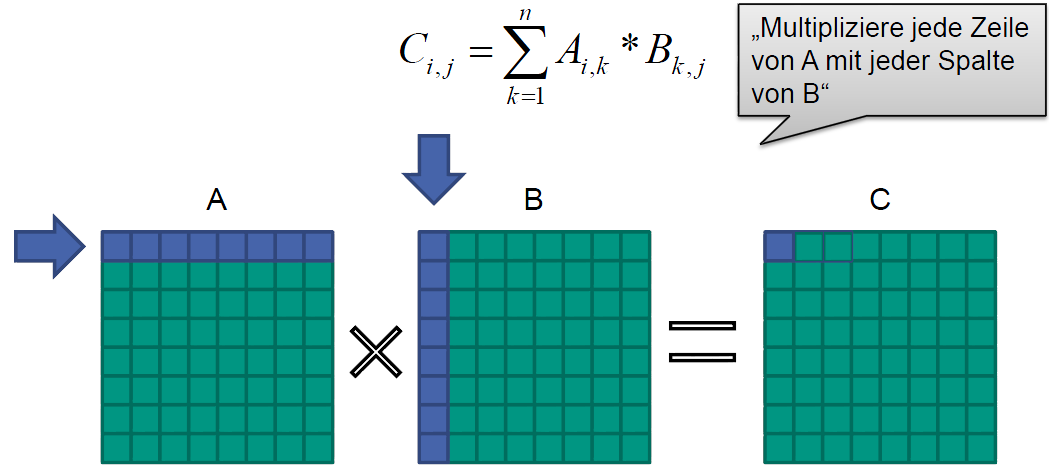
\includegraphics[width=\textwidth]{pics/06/matrix_klassisch}
	\end{center}
	Problem: cache-unfreundlich
	\end{block}
}

\begin{frame}[fragile]
\frametitle {Matrix-Matrix-Multiplikation} 
	\begin{block} {Quellcode zu ``ijk''}

	\begin{lstlisting} {}
public int[][] matrixMult (int[][] a, int[][] b) {
  final int N = a.length;
  int[][] c = new int[N][N];
  
  for(int i = 0; i < N; i++) {
    for(int j = 0; j < N; j++) {
      for(int k = 0; k < N; k++) {
        c[i][j] += a[i][k] * b[k][j];
      }
    }
  }
  return c;
}
	\end{lstlisting}
	\end{block} 
\end{frame}

\begin{frame}[fragile]
\frametitle {Matrix-Matrix-Multiplikation} 
	\begin{block} {Quellcode zu ``ikj''}
durch Neuordnung der Schleifen wird ein Operand schleifeninvariant \pause
	\begin{lstlisting} {}
for(i=0; i < N; i++)
  for(k=0; k < N; k++)
    for(j=0; j < N; j++)
      c[i][j] += a[i][k] * b[k][j];
	\end{lstlisting}
der invariante Teil muss nur einmal berechnet werden \pause
	\begin{lstlisting} {}
for(i=0; i < N; i++)
  for(k=0; k < N; k++) {
    r = a[i][k];
    for(j=0; j < N; j++)
      c[i][j] += r* b[k][j];
  }
	\end{lstlisting}
	\end{block} 
\end{frame}

\frame {
\frametitle {Matrix-Matrix-Multiplikation} 
	\begin{center}
	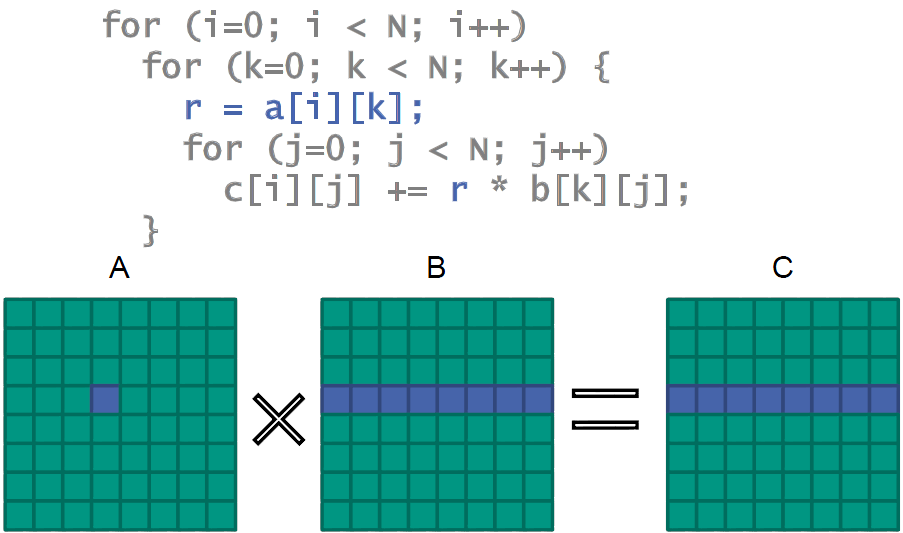
\includegraphics[width=0.6\textwidth]{pics/06/matrix_ikj}
	\end{center}
	\begin{block} {ikj-Algorithmus}
	\begin{itemize}
		\item cache-freundlich \pause
		\item weniger parallelisierbar als ijk - weshalb?
		\visible<3-> {
		\item es können nur noch die $N$ Iterationen der äußeren Schleife parallel ohne Synchronisation für C bearbeitet werden
		}
	\end{itemize}

	\end{block}
}

\section{Klausuraufgaben}
\begin{frame}[fragile]
\frametitle {Klausur 2010-1} 
	\begin{block} {A3 b)}
	Ergänzen Sie den folgenden Quelltext der Klasse \texttt{Singleton}, so dass sie das Entwurfsmuster ``Einzelstück'' implementiert. Zudem soll Ihre Implementierung für die mehrfädige Ausführung geeignet sein. Verwenden Sie korrekte Java-Syntax. (3 P)
	\end{block}
	
	\begin{lstlisting} {}
/**
 * Implementiert ein fuer mehrfaedige Programme 
 * geeignetes Einzelstueck
 */
public class Singleton {



}
	\end{lstlisting}
\end{frame}

\section{Klausuraufgaben}
\begin{frame}[fragile]
\frametitle {Klausur 2010-1 A3 b) Lösung} 
	
	\begin{lstlisting} {}
public class Singleton {
  // Instanzvariable Einzelstuecks
  private static Singleton instanz = null;
  
  // Default-Konstruktor privat deklarieren
  private Singleton() {}
  
  // Statische Methode, die die Instanz zurueckgibt
  public static synchronized Singleton getInstance() {
    if (instanz == null) {
      instanz = new Singleton();
  }
  return instanz;
}
	\end{lstlisting}
\end{frame}

\frame {
\frametitle {Klausuraufgaben zum Aufwärmen} 
	\begin{block} {Aufgabe 1 (2,5P)}
	Nennen Sie 5 aus der Vorlesung bekannte Prozessmodelle zur Softwareentwicklung.\\
	\begin{itemize}
		\visible<2-> {
		\item Programmieren durch Probieren
		\item Wasserfallmodell
		\item V-Modell
		\item Prototypenmodell
		\item Iteratives Modell
		\item Synchronisiere und Stabilisiere
		\item Agile Methoden (spez. Extreme Programming)
		}
	\end{itemize}
	\end{block}
}

\frame {
\frametitle {Klausuraufgaben zum Aufwärmen} 
	\begin{block} {Aufgabe 2 (2P)}
		Nennen Sie 2 aus der Vorlesung bekannte Basismethoden der Aufwandsschätzung und erklären Sie eine davon kurz. \\
		\begin{itemize}
		\visible<2-> {
			\item Analogiemethode
			\item Relationsmethode
			\item Multiplikatormethode
			\item Phasenaufteilung
			}
		\end{itemize}
	\end{block}
}

\frame {
\frametitle {Klausuraufgaben zum Aufwärmen} 
	\begin{block} {Aufgabe 2 (3P)}
		Nennen Sie die 3 aus der Vorlesung bekannten Arten von Testhelfern und erklären Sie diese jeweils in einem Satz. \\
		\begin{itemize}
		\visible<2-> {
			\item Stummel (stub)  \visible<3-> {Rudimentär implementierte Methode als Teil der Software. Dient als Platzhalter für 	noch nicht umgesetzte Funktionalität.}
			\item Attrappe (dummy):  \visible<4->{Simuliert die Implementierung zu Testzwecken}
			\item Nachahmung (mock):  \visible<5->{Attrappe mit zusätzlicher Funktionalität, wie bspw. das Einstellen der Reaktion der Nachahmung auf bestimmte Eingaben oder das Überprüfen des Verhaltens des „Klienten“.}
			}
		\end{itemize}
	\end{block}
}

\section{inoffizielle Probeklausur}

\frame{
\frametitle{inoffizielle Probeklausur}

	\begin{block}{Ablauf}
	\begin{itemize}
	\item Zeit: 25.7. 18 Uhr \pause
	\item Ort: Audimax
	\item die Tutoren korrigieren die Probeklausuren \pause
	\item Rückgabe in der gleichen Woche, vorraussichtlich Freitag \pause
	\item die Probeklausur wird von Tutoren ausgerichtet, es gibt keinen Zusammenhang mit der offizellen Klausur!
	\end{itemize}
	\end{block}
\pause
	\begin{block}{Anmeldung}
	\begin{itemize}
	\item damit wir genügend Kopien drucken können, meldet euch bitte jetzt an \pause
	\item damit die Probeklausur euch hilft, müsst ihr schon vorher mit der Klausurvorbereitung anfangen
	\end{itemize}
	\end{block}
}


\frame{
\frametitle{Bis zum nächsten Mal}
	\begin{center}
	
\includegraphics[height=200pt]{pics/06/06_comic}
	\end{center}
}

\end{document}
